\documentclass[12pt]{article}

\usepackage{fontawesome}
\usepackage{hyperref}
\usepackage{xurl}
\usepackage{fancyvrb}
\usepackage{graphicx}
\usepackage{float}
\usepackage[tagged, highstructure]{accessibility}
\usepackage{bookmark}
\usepackage{enumitem}

\hypersetup{
    colorlinks=false,
    pdfborder={0 0 0},
    pdftitle={Query Optimization},
    pdfauthor={Adrianna Holden-Gouveia},
    pdfsubject={Advanced Data - Lab Assignment},
    pdflang={en-US},
    pdfkeywords={query optimization, indexes, performance, SQL, Kaggle}
}

% Configure PDF bookmarks for navigation
\bookmarksetup{
    numbered,
    open,
}

% Configure list spacing for better accessibility
\setlist{nosep}



\title{Query Optimization}
\author{
        Adrianna Holden-Gouveia \\
        Website: \href{https://aholdengouveia.name}{aholdengouveia.name}\\ 
        \date{\vspace{-5ex}}
        %Email: \href{mailto:admin@aholdengouveia.name}{admin@aholdengouveia.name} \\
%        \faLinkedin{: aholdengouveia} \\
        \faGithub {: aholdengouveia} \\
        %\faTwitter {: aholdengouveia} \\
        }

%S\date{\today}


\begin{document}    

\maketitle

%\begin{abstract}
%This is a template for Linux Administration Lab work
%\end{abstract}
%\tableofcontents


\section*{Accessibility Notice}
This document is also available in HTML format at:

Link: \href{https://aholdengouveia.name/AdvData/labs/week5optimization.html}{\textbf{\nolinkurl{https://aholdengouveia.name/AdvData/labs/week5optimization.html}}}

The HTML version provides enhanced accessibility features including keyboard navigation, screen reader support, responsive design, dark mode support, and high contrast options.

\section*{Request}
\noindent\textbf{Request:} DATA-7391\\
\textbf{Requested by:} Help desk\\
\textbf{Data:} My book database, then your own database

\section*{Background}
Users have started reporting that some searches are slow. Your manager wants you to learn how to find and fix slow queries by practising on a sample database, then check your own queries and write up a fix so the team can approve it. On a real system with millions of rows, a missing index can turn a search that takes seconds into one that takes minutes.

\section*{Learning Outcomes}
By the end of this lab, you will be able to:
\begin{itemize}
    \item Read a query plan, and explain how an index changes it
    \item Write commands that add an index to a table for a specific query
    \item Optimize your own SQL queries, and decide whether an index is worth it
    \item Write up a performance fix with evidence, the way you would for a work ticket
\end{itemize}

\section*{Lab Instructions}
Parts 3 and 4 use your own data set and the queries you documented in the SQL Review labs. If you want to switch to a different data set, email me first. Switching means redoing the work from earlier labs for your new data set, so it adds a lot of work. The switching checklist (linked under Resources) lists what you'd need to redo.

\subsection*{Screenshots}
Several parts of this lab ask for a screenshot. Each screenshot should have your name, term, and year.  One of the easiest ways to do that is make a text document with your name and term/year on your computer and save it to use all term. Any screenshots that don't include this information won't be counted.

\begin{figure}[H]
    \centerline{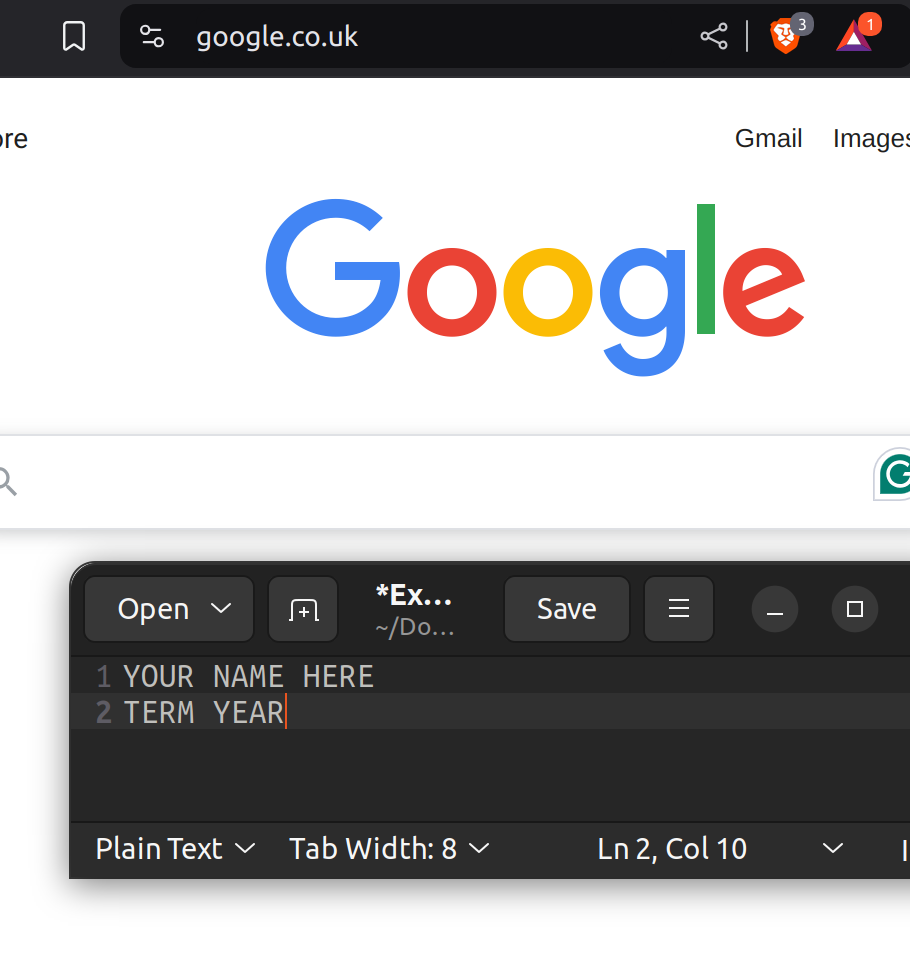
\includegraphics[scale=.2]{ExampleScreenshot.png}}
    \caption{This is an image of what each of your screenshots should look like}
    \alt{Example screenshot: a web browser showing the Google home page, with a small text editor window in front of it that says YOUR NAME HERE and TERM YEAR}
\end{figure}

\subsection*{Part 1: Writing Efficient Queries on Kaggle}
Sign up for Kaggle (linked under Resources). It's free, and you can use any email you want. You only need the Writing Efficient Queries lesson from Kaggle's Advanced SQL course, not the whole course.
\begin{enumerate}
    \item Read the Writing Efficient Queries tutorial.
    \item Do the Writing Efficient Queries exercise. It has problems about Pet Costumes International. Take a screenshot of your solution to both problems.
    \item In a few sentences, explain one technique from the tutorial that makes a query more efficient, and why it helps.
\end{enumerate}
Kaggle uses BigQuery, which doesn't use indexes the way most databases do, so this part is about writing efficient queries. Parts 2 and 3 are about indexes.

\textbf{Optional, not required for this class:} if you're interested, the rest of Kaggle's Advanced SQL course covers joins and unions, analytic functions, and nested data.

\subsection*{Part 2: Indexes and Query Plans}
Load my book database (linked under Resources) into any SQLite tool. I suggest SandboxSQL, linked under Resources: use Load a Database, then load the .sqlite file. Queries don't always copy over well from a PDF, especially single quotes, so type them in if you get an error.

\textbf{How to read a query plan:} put EXPLAIN QUERY PLAN in front of any query, and the database tells you how it will find the rows, without running the query. Look for these two words:
\begin{itemize}
    \item SCAN means the database reads every row in the table. On a big table, this is slow.
    \item SEARCH ... USING INDEX means the database uses an index to go straight to the rows it needs.
\end{itemize}
The exact wording can be a little different depending on your tool, but SCAN and SEARCH will be there.

\textbf{Worked example:} this query finds books by one publisher.
\begin{Verbatim}
EXPLAIN QUERY PLAN
SELECT title, publishDate FROM books
WHERE publisher = 'Penguin Books';
\end{Verbatim}
Before an index, the plan says SCAN books. Then I create an index on the column in the WHERE:
\begin{Verbatim}
CREATE INDEX idx_books_publisher ON books(publisher);
\end{Verbatim}
Running the same EXPLAIN QUERY PLAN again now says SEARCH books USING INDEX \nolinkurl{idx_books_publisher}. Follow the same steps for the questions below.

\begin{enumerate}
    \item This query finds the author and genre of a book with a given title.
    \begin{Verbatim}
SELECT authors.name, books.genre
FROM books INNER JOIN authors
ON books.author_id = authors.author_id
WHERE books.title = 'Dune';
    \end{Verbatim}
    \begin{enumerate}
        \item Run EXPLAIN QUERY PLAN on it, and take a screenshot of the plan.
        \item Write and run the command that creates an index to make this query more efficient.
        \item Run EXPLAIN QUERY PLAN again, and take a screenshot. Explain what changed in the plan and why that makes the query faster.
    \end{enumerate}
    \item Create an index on the genre column. Then write a query that shows only Fantasy books, with the author's name and the title. Run EXPLAIN QUERY PLAN on your query and take a screenshot that shows your index being used. If your plan still says SCAN books, check that your WHERE uses = with the indexed column. A LIKE that starts with \% can't use an index.
    \item Indexes aren't free. They take up space, and they make adding or changing rows slower. Pick a column in your own data set that would be a bad choice for an index, and explain why. For example, think about columns that are rarely searched, have only a few different values, or change often.
\end{enumerate}

\subsection*{Part 3: Optimize Your Own Queries}
Pick 2 of your documented queries from the SQL Review labs. For each one:
\begin{enumerate}
    \item Run EXPLAIN QUERY PLAN on it, and take a screenshot.
    \item Decide whether an index would help. If it would, create it, run EXPLAIN QUERY PLAN again, and take a screenshot.
    \item Update the Notes in your query documentation with what the plan showed, any index you created, and whether it was worth it.
\end{enumerate}
Your data set may be small, so you probably won't see a difference in time. The plan is your evidence. If you decide an index isn't worth it, that's a fine answer, as long as you explain why.

\subsection*{Part 4: Performance Ticket Write-Up}
A user reports that one of your queries from Part 3 is slow. Write up the fix for your team lead, following the sample performance ticket (linked under Resources). Include the problem, the query, what you checked, what you changed, your evidence, the trade-offs, how to undo the change, and your recommendation.

\section*{Acceptance Criteria}
This request is done when:
\begin{itemize}
    \item Both problems in the Kaggle Writing Efficient Queries exercise are solved, and you've explained one technique from the tutorial
    \item Every index you create has a query plan from before and after as evidence
    \item Your genre query plan shows your index being used
    \item 2 of your own queries are checked, with an explanation of whether an index is worth it
    \item Your performance ticket write-up includes everything in the sample, including how to undo the change
    \item Every screenshot follows the screenshot rules
\end{itemize}

\section*{Deliverables}
One file that includes:
\begin{itemize}
    \item Part 1: your 2 Kaggle screenshots and your explanation of one technique
    \item Part 2: your answers, commands, queries, and plan screenshots
    \item Part 3: your 2 updated query documentations with plan screenshots
    \item Part 4: your performance ticket write-up
    \item If you switched data sets: the redone work from the switching checklist
\end{itemize}

Audience: your team lead, who has to approve the change.

\section*{Resources}
References, a video, a PowerPoint and some notes are available at my website
Link: \href{https://www.aholdengouveia.name/AdvData/optimization.html}{\textbf{\nolinkurl{https://www.aholdengouveia.name/AdvData/optimization.html}}}

Kaggle Writing Efficient Queries tutorial
Link: \href{https://www.kaggle.com/code/alexisbcook/writing-efficient-queries}{\textbf{\nolinkurl{https://www.kaggle.com/code/alexisbcook/writing-efficient-queries}}}

Kaggle Writing Efficient Queries exercise
Link: \href{https://www.kaggle.com/code/alexisbcook/exercise-writing-efficient-queries}{\textbf{\nolinkurl{https://www.kaggle.com/code/alexisbcook/exercise-writing-efficient-queries}}}

Optional: the full Kaggle Advanced SQL course
Link: \href{https://www.kaggle.com/learn/advanced-sql}{\textbf{\nolinkurl{https://www.kaggle.com/learn/advanced-sql}}}

My book database for Part 2
Link: \href{https://www.aholdengouveia.name/AdvData/labs/BooksDatabase.sqlite}{\textbf{\nolinkurl{https://www.aholdengouveia.name/AdvData/labs/BooksDatabase.sqlite}}}

Suggested tool: SandboxSQL, free, runs in your browser, and saves your database as a .sqlite file with its Export button
Link: \href{https://www.sandboxsql.com/}{\textbf{\nolinkurl{https://www.sandboxsql.com/}}}

Optional, if you'd rather install a tool: DB Browser for SQLite, which can import a CSV file directly
Link: \href{https://sqlitebrowser.org/}{\textbf{\nolinkurl{https://sqlitebrowser.org/}}}

SQLite documentation on EXPLAIN QUERY PLAN
Link: \href{https://www.sqlite.org/eqp.html}{\textbf{\nolinkurl{https://www.sqlite.org/eqp.html}}}

Use The Index, Luke: a guide to indexes for developers
Link: \href{https://use-the-index-luke.com/}{\textbf{\nolinkurl{https://use-the-index-luke.com/}}}

Sample query documentation
Link: \href{https://www.aholdengouveia.name/AdvData/labs/SampleQueryDocumentation.txt}{\textbf{\nolinkurl{https://www.aholdengouveia.name/AdvData/labs/SampleQueryDocumentation.txt}}}

Sample performance ticket write-up for Part 4
Link: \href{https://www.aholdengouveia.name/AdvData/labs/SamplePerformanceTicket.txt}{\textbf{\nolinkurl{https://www.aholdengouveia.name/AdvData/labs/SamplePerformanceTicket.txt}}}

Switching checklist, if you want to change data sets
Link: \href{https://www.aholdengouveia.name/AdvData/labs/SwitchingDataSets.txt}{\textbf{\nolinkurl{https://www.aholdengouveia.name/AdvData/labs/SwitchingDataSets.txt}}}

\end{document}